\documentclass[10pt, aspectratio=169]{beamer}

% Theme and styling setup
\usetheme{Madrid}
\usecolortheme{whale}

% Font and language configuration
\usepackage{fontspec}
\usepackage[german]{babel}
\usepackage{amsmath}
\usepackage{booktabs}
\usepackage{unicode-math}
\usepackage{graphicx}

% Color definitions
\definecolor{maincolor}{RGB}{30, 58, 138}    % Deep Navy Blue
\definecolor{accentcolor}{RGB}{13, 148, 136}  % Teal Accent
\definecolor{bglight}{RGB}{248, 250, 252}     % Slate Light Gray

\setbeamercolor{palette primary}{bg=maincolor, fg=white}
\setbeamercolor{palette secondary}{bg=accentcolor, fg=white}
\setbeamercolor{structure}{fg=maincolor}
\setbeamercolor{frametitle}{bg=maincolor, fg=white}
\setbeamercolor{block title}{bg=maincolor, fg=white}
\setbeamercolor{block body}{bg=bglight, fg=black}

\title[Passwortsicherheit]{Passwortsicherheit, Entropie \& Best Practices}
\subtitle{Informatik | Kantonsschule im Lee}
\author{Laurin Ott}
\date{2. November 2026}

\begin{document}

% -----------------------------------------------------------------------------
% TITLE SLIDE
% -----------------------------------------------------------------------------
\begin{frame}
  \titlepage
\end{frame}

% -----------------------------------------------------------------------------
% LEKTION 1: HOOK & THOUGHT EXPERIMENT
% -----------------------------------------------------------------------------
\begin{frame}{Einstieg: Welches Passwort ist sicherer?}
  \begin{columns}[c]
    \begin{column}{0.48\textwidth}
      \begin{alertblock}{Passwort A}
        \centering \Large \textbf{Sh5?L@}
        \vspace{0.3em}
        \small
        \begin{itemize}
          \item Länge: $L = 6$
          \item Enthält Gross-/Kleinbuchstaben, Zahlen \& Sonderzeichen
        \end{itemize}
      \end{alertblock}
    \end{column}
    
    \begin{column}{0.48\textwidth}
      \begin{exampleblock}{Passwort B}
        \centering \Large \textbf{kamelregentischblauargentinienschule}
        \vspace{0.3em}
        \small
        \begin{itemize}
          \item Länge: $L = 36$
          \item Nur Kleinbuchstaben
        \end{itemize}
      \end{exampleblock}
    \end{column}
  \end{columns}

  \vspace{1.5em}
  \centering
  \textbf{Frage an die Klasse:} \textit{Welches Passwort hält einem Computerangriff länger stand und welches lässt sich besser merken?}
\end{frame}

% -----------------------------------------------------------------------------
% AGENDA SLIDE
% -----------------------------------------------------------------------------
\begin{frame}{Ablauf \& Zeitplan}
  \begin{columns}[T]
    \begin{column}{0.48\textwidth}
      \begin{block}{Lektion 1 (45 Min.)}
        \small
        \begin{itemize}
          \item \textbf{00--02 min:} Vorstellung \& Warum ich hier bin
          \item \textbf{02--04 min:} Brute-Force Demo
          \item \textbf{04--06 min:} Abstimmung: Welches Passwort besser?
          \item \textbf{06--08 min:} Voting aufgelöst
          \item \textbf{08--23 min:} Entropie erklären (15 Min.)
          \item \textbf{23--38 min:} Aufgaben rechnen (15 Min.)
          \item \textbf{38--45 min:} Ende gerechnet / Besprechung
        \end{itemize}
      \end{block}
    \end{column}
    \begin{column}{0.48\textwidth}
      \begin{block}{Lektion 2 (45 Min.)}
        \small
        \begin{itemize}
          \item \textbf{00--05 min:} Start 2. Lektion / Diceware
          \item \textbf{05--15 min:} Nist Best Practices / MFA / Passwort-Manager
          \item \textbf{15--20 min:} Best Practices und MFA übungen (5 Min.)
          \item \textbf{20--30 min:} Aufgabe: HIBP \& Passwortcheck (10 Min.)
          \item \textbf{30--45 min:} Umfrage ausfüllen (15 Min.)
          \item \textbf{Rest Zeit:}  Artikel Passwort-Manager \& Passwortspiel
        \end{itemize}
      \end{block}
    \end{column}
  \end{columns}
\end{frame}

% -----------------------------------------------------------------------------
% ANGRIFFSARTEN
% -----------------------------------------------------------------------------
\begin{frame}{Wie greifen Computer Passwörter an?}
  \begin{block}{1. Brute-Force-Angriff}
    Ein automatisierter Angriff, bei dem Programme \textbf{systematisch alle möglichen Zeichenkombinationen} durchprobieren ($a, b, c \dots aa, ab \dots$).
  \end{block}

  \vspace{0.8em}

  \begin{block}{2. Dictionary Attack (Wörterbuchangriff)}
    Ein gezielter Angriff, bei dem Listen mit \textbf{gebräuchlichen Wörtern, Namen, Daten und bekannten Passwörtern} durchgetestet werden.
  \end{block}

  \vspace{0.8em}
  \textbf{Das Problem menschlicher Eingaben:} Wir wählen vorhersehbare Muster (\textit{z. B. Jahreszahlen, Grossbuchstabe am Anfang}). Der tatsächliche Suchraum für Angreifer schrumpft dadurch drastisch!
\end{frame}


% -----------------------------------------------------------------------------
% MFA (MULTI-FACTOR AUTHENTICATION)
% -----------------------------------------------------------------------------
\begin{frame}{Multifaktor-Authentifizierung}
  \begin{block}{Was ist MFA?}
    Multi-Faktor-Authentifizierung (MFA) ist ein Sicherheitsverfahren, bei dem Benutzer \textbf{mehrere unabhängige Faktoren}(z.\,B. Einmalcode oder App-Bestätigung) zur Verifizierung ihrer Identität bereitstellen müssen. MFA ist extrem effektiv, da Passwörter alleine für eine erfolgreiche Übernahme meist nicht ausreichen. 
  \end{block}

  \vspace{0.8em}
  \textbf{Vorteil:} Selbst wenn ein Angreifer Ihr Passwort kennt, kann er ohne den zweiten Faktor nicht auf Ihr Konto zugreifen.
\end{frame}

% -----------------------------------------------------------------------------
% MATHEMATISCHE GRUNDLAGE: ENTROPIE
% -----------------------------------------------------------------------------
\begin{frame}{Die mathematische Grundlage: Shannon-Entropie}
  \begin{block}{Was ist die Entropie ($E$)?}
    Die Shannon-Entropie misst den Grad der \textbf{Zufälligkeit} bei der Passwort-Generierung in der Einheit \textbf{Bit}. 1 Bit entspricht einer binären Ja/Nein-Entscheidung ($1/0$).
  \end{block}

  \vspace{0.5em}

  \begin{columns}[T]
    \begin{column}{0.48\textwidth}
      \textbf{Für Zeichen-Passwörter:}
      \[ N = R^L \]
      \[ E = \log_2(N) = L \cdot \log_2(R) \]
    \end{column}
    \begin{column}{0.48\textwidth}
      \textbf{Für Wort-Passphrasen:}
      \[ N = W^L \]
      \[ E = \log_2(N) = L \cdot \log_2(W) \]
    \end{column}
  \end{columns}

  \vspace{0.8em}
  \small
  \begin{itemize}
    \item $L$: Länge (Anzahl Zeichen bzw. Wörter)
    \item $R$: Größe des Zeichensatzes (z. B. $R=26$ für Kleinbuchstaben, $R=94$ für alle Zeichen)
    \item $W$: Anzahl der Wörter im Wörterbuch (z. B. $W=7776$ bei Diceware)
  \end{itemize}
\end{frame}

% -----------------------------------------------------------------------------
% BEISPIELRECHNUNG (AUFGABE 5)
% -----------------------------------------------------------------------------
\begin{frame}{Rechnen an der Tafel: Komplexität vs. Länge}
  \begin{columns}[T]
    \begin{column}{0.48\textwidth}
      \begin{block}{Szenario A: Kurze Komplexität}
        \begin{itemize}
          \item Länge: $L = 8$
          \item Zeichensatz: Alle Zeichen ($R = 94$)
        \end{itemize}
        \[ E_A = 8 \cdot \log_2(94) \approx \mathbf{52{,}4\text{ Bit}} \]
      \end{block}
    \end{column}

    \begin{column}{0.48\textwidth}
      \begin{block}{Szenario B: Lange Einfachheit}
        \begin{itemize}
          \item Länge: $L = 20$
          \item Zeichensatz: Nur Kleinbuchstaben ($R = 26$)
        \end{itemize}
        \[ E_B = 20 \cdot \log_2(26) \approx \mathbf{94{,}0\text{ Bit}} \]
      \end{block}
    \end{column}
  \end{columns}

  \vspace{1.2em}
  \begin{alertblock}{Mathematisches Fazit}
    Die Anzahl Möglichkeiten $N = R^L$ wächst \textbf{exponentiell} mit der Länge ($L$), aber nur \textbf{logarithmisch} mit dem Zeichensatz ($R$). \textbf{Länge schlägt Komplexität!}
  \end{alertblock}
\end{frame}

% -----------------------------------------------------------------------------
% ENTROPIE TABELLE
% -----------------------------------------------------------------------------
\begin{frame}{Übersicht: Entropie für verschiedene Längen \& Zeichensätze}
  \centering
  \small
  \begin{tabular}{l c l r}
    \toprule
    \textbf{Zeichensatz ($R$)} & \textbf{Länge ($L$)} & \textbf{Formel} & \textbf{Entropie ($E$)} \\
    \midrule
    Kleinbuchstaben ($R=26$) & 8 & $8 \cdot \log_2(26)$ & $\approx 37{,}6$ Bit \\
    Alle Zeichen ($R=94$) & 8 & $8 \cdot \log_2(94)$ & $\approx 52{,}4$ Bit \\
    Kleinbuchstaben ($R=26$) & 16 & $16 \cdot \log_2(26)$ & $\approx 75{,}2$ Bit \\
    Kleinbuchstaben ($R=26$) & 20 & $20 \cdot \log_2(26)$ & $\approx 94{,}0$ Bit \\
    Alle Buchstaben ($R=52$) & 20 & $20 \cdot \log_2(52)$ & $\approx 114{,}0$ Bit \\
    Alle Zeichen ($R=94$) & 20 & $20 \cdot \log_2(94)$ & $\approx 131{,}1$ Bit \\
    \bottomrule
  \end{tabular}
  
  \vspace{1em}
  \textit{Hinweis: Umrechnung auf wissenschaftlichen Taschenrechnern: $\log_2(x) = \frac{\ln(x)}{\ln(2)} = \frac{\log(x)}{\log(2)}$}
\end{frame}

% -----------------------------------------------------------------------------
% WORKPHASE ANNOUNCEMENT
% -----------------------------------------------------------------------------
\begin{frame}{Arbeitsphase: Aufgabenblatt 1 (Teil 1 \& 2)}
  \begin{center}
    \Large \textbf{Jetzt sind Sie dran!}
  \end{center}

  \vspace{1em}
  \begin{block}{Arbeitsauftrag (15 Minuten in Partnerarbeit)}
    \begin{enumerate}
      \item Öffnet euer Skript auf \textbf{Seite 7} (Abschnitt 3.1).
      \item Lösen Sie die \textbf{Aufgaben 1 und 3 bis 5} zur Entropieberechnung.
      \item Nutzen Sie den Taschenrechner für die Logarithmen oder benutzen Sie das Entropierechner-Tool auf Moodle!
    \end{enumerate}
  \end{block}
\end{frame}

% -----------------------------------------------------------------------------
% DICEWARE
% -----------------------------------------------------------------------------
\begin{frame}{Das Diceware-Verfahren}
  \begin{columns}[c]
    \begin{column}{0.6\textwidth}
      \textbf{Wie generiert man echte Zufalls-Passphrasen?}
      \begin{enumerate}
        \item Würfelen Sie $5\times$ mit einem normalen 6-seitigen Würfel (z. B. 3-2-5-4-1).
        \item Schlagen Sie das Wort in der Diceware-Liste(auf Moodle) nach ($W=7776$ Wörter).
        \item Wiederholen Sie das für 5 bis 7 Wörter.
      \end{enumerate}
    \end{column}
    \begin{column}{0.38\textwidth}
      \begin{block}{Klassen-Passphrase}
        Bei 7 gewürfelten Wörtern:
        \[ E = 7 \cdot \log_2(7776) \]
        \[ E \approx \mathbf{90{,}5\text{ Bit}} \]
        \textit{Praktisch unknackbar!}
      \end{block}
    \end{column}
  \end{columns}
\end{frame}

% -----------------------------------------------------------------------------
% LEKTION 2: HANDS-ON TOOL CHECK
% -----------------------------------------------------------------------------
\begin{frame}{Lektion 2: Hands-On Praxis-Check}
  \begin{block}{Auftrag (10 Minuten am Laptop)}
    Öffnet die folgenden zwei Sicherheits-Tools und testet fiktive Beispiele:
  \end{block}

  \vspace{0.8em}
  
  \begin{columns}[T]
    \begin{column}{0.48\textwidth}
      \textbf{1. passwortcheck.ch}
      \begin{itemize}
        \item Testen Sie verschiedene Muster (z.B. \texttt{Sommer2026!} vs. gewürfelte Passphrasen).
        \item \textit{Achtung:} Geben Sie niemals Ihre echten Passwörter ein!
      \end{itemize}
    \end{column}

    \begin{column}{0.48\textwidth}
      \textbf{2. haveibeenpwned.com}
      \begin{itemize}
        \item Gehen Sie auf \texttt{haveibeenpwned.com/Passwords} und testen Sie einige häufige Passwörter (z. B. \texttt{123456} oder \texttt{Passwort1}), um zu sehen, wie oft es geleakt wurde.
        \item Scrollen Sie auf der Startseite herunter, welche bekannten Websiten/Plattformen hatten bereits grosse Datenlecks?
        \item (Freiwillig) Prüfen Sie mit eurer E-Mail-Adresse, ob ihr selbst von einem Datenleck betroffen wart.
      \end{itemize}
    \end{column}
  \end{columns}
\end{frame}

% -----------------------------------------------------------------------------
% BEST PRACTICES (NIST)
% -----------------------------------------------------------------------------
\begin{frame}{Die 4 goldenen Regeln der Passwortsicherheit (NIST)}
  \begin{block}{1. Länge vor Komplexität}
    Bevorzugung von Passphrasen aus mehreren zufälligen Wörtern.
  \end{block}

  \begin{block}{2. Keine Wiederverwendung von Passwörtern}
    Jedes Konto benötigt ein einzigartiges Passwort (Schutz bei Datenlecks!).
  \end{block}

  \begin{block}{3. Keine erzwungenen Änderungen ohne Anlass}
    Regelmässige Passwortwechsel führen zu schwächeren Mustern und Eselsbrücken.
  \end{block}

  \begin{block}{4. Passwort-Manager \& MFA nutzen}
    Zufällige Passwörter verwalten lassen und den 2. Faktor aktivieren.
  \end{block}
\end{frame}

% -----------------------------------------------------------------------------
% FEEDBACK / CONCLUSION
% -----------------------------------------------------------------------------
\begin{frame}{Unterrichts-Feedback}
  \begin{center}
    \Large \textbf{Vielen Dank für eure aktive Mitarbeit!}
    
    \vspace{1.5em}
    \normalsize
    Bitte scannen Sie den QR-Code an der Wandtafel oder nutzen den Link (auf Moodle), um mir ein kurzes Feedback zu den beiden Lektionen zu geben. Wenn Sie noch Fragen haben, stellen Sie diese bitte jetzt.
    \center
    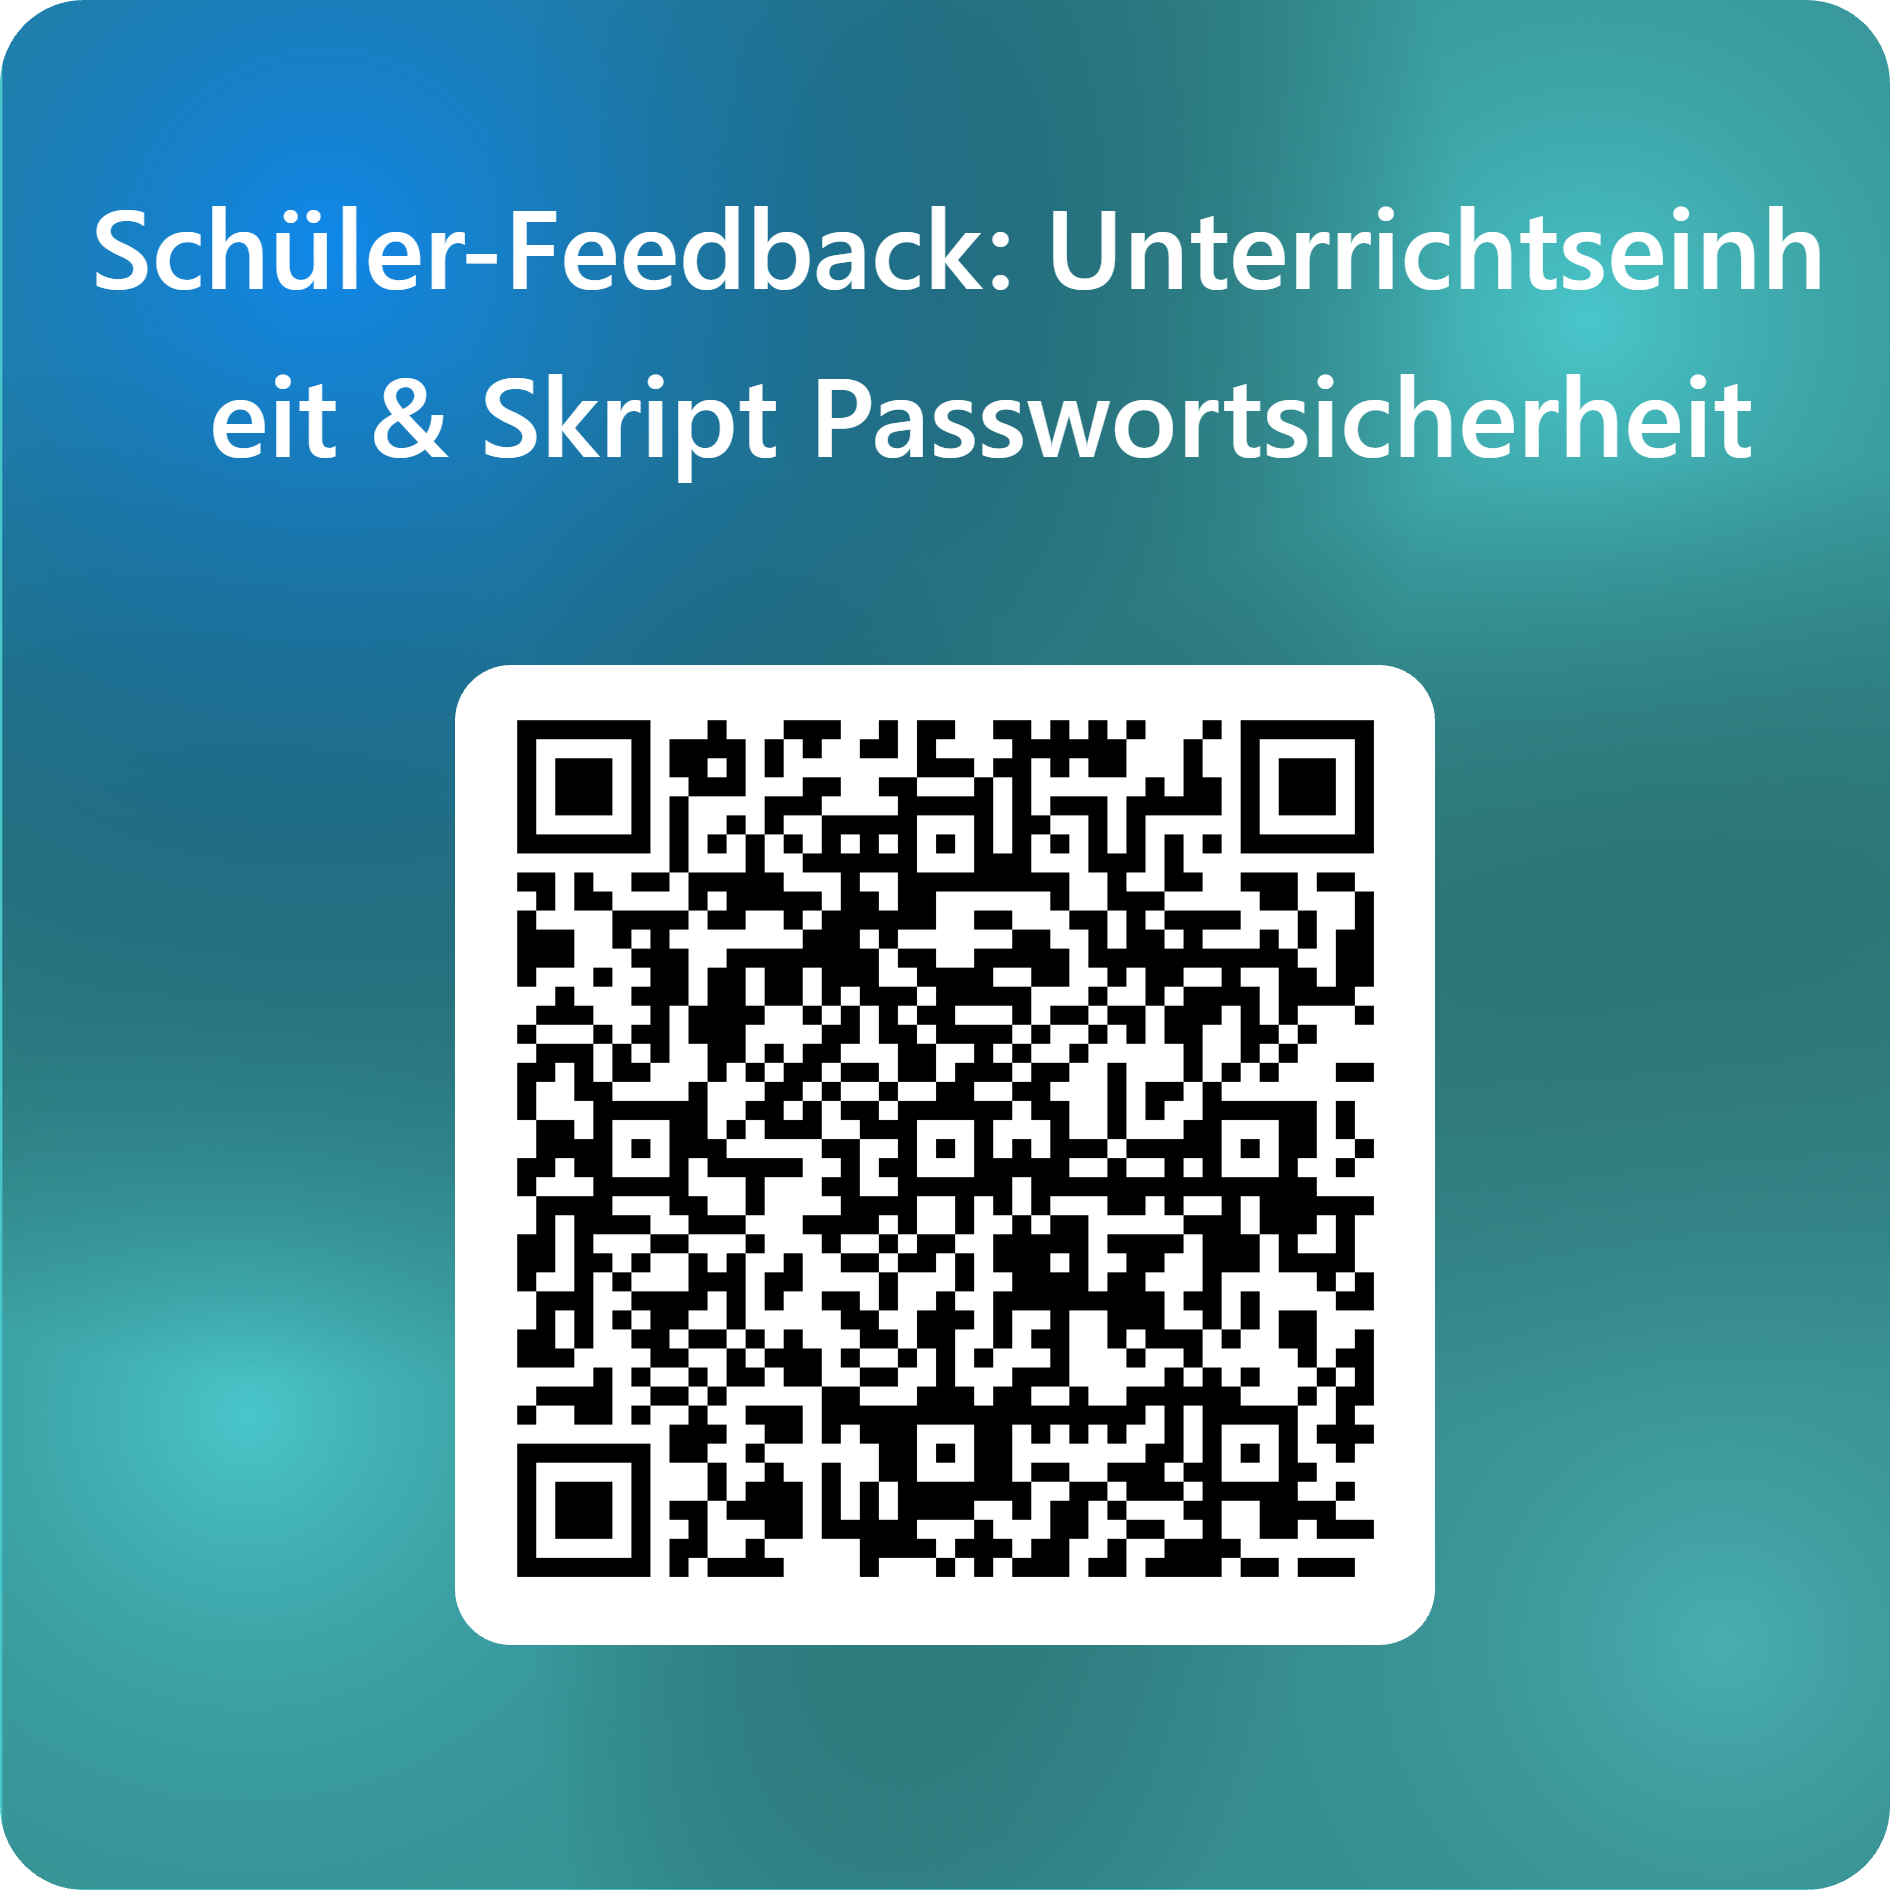
\includegraphics[width=0.3\textwidth]{QRCode Feedback Passwortsicherheit.png}
  \end{center}
\end{frame}

\end{document}